\documentclass[a4paper]{report}
% Some basic packages
\usepackage[utf8]{inputenc}
\usepackage[T1]{fontenc}
\usepackage{textcomp}
\usepackage[english]{babel}
\usepackage{url}
\usepackage{graphicx}
\usepackage{float}
\usepackage{booktabs}
\usepackage{enumitem}

\pdfminorversion=7

% Don't indent paragraphs, leave some space between them
\usepackage{parskip}

% Hide page number when page is empty
\usepackage{emptypage}
\usepackage{subcaption}
\usepackage{multicol}
\usepackage{xcolor}

% Other font I sometimes use.
% \usepackage{cmbright}

% Math stuff
\usepackage{amsmath, amsfonts, mathtools, amsthm, amssymb}
% Fancy script capitals
\usepackage{mathrsfs}
\usepackage{cancel}
% Bold math
\usepackage{bm}
% Some shortcuts
\newcommand\N{\ensuremath{\mathbb{N}}}
\newcommand\R{\ensuremath{\mathbb{R}}}
\newcommand\Z{\ensuremath{\mathbb{Z}}}
\renewcommand\O{\ensuremath{\emptyset}}
\newcommand\Q{\ensuremath{\mathbb{Q}}}
\newcommand\C{\ensuremath{\mathbb{C}}}
\renewcommand\L{\ensuremath{\mathcal{L}}}

% Package for Petri Net drawing
\usepackage[version=0.96]{pgf}
\usepackage{tikz}
\usetikzlibrary{arrows,shapes,automata,petri}
\usepackage{tikzit}
\input{petri_nets_style.tikzstyles}

% Easily typeset systems of equations (French package)
\usepackage{systeme}

% Put x \to \infty below \lim
\let\svlim\lim\def\lim{\svlim\limits}

%Make implies and impliedby shorter
\let\implies\Rightarrow
\let\impliedby\Leftarrow
\let\iff\Leftrightarrow
\let\epsilon\varepsilon

% Add \contra symbol to denote contradiction
\usepackage{stmaryrd} % for \lightning
\newcommand\contra{\scalebox{1.5}{$\lightning$}}

% \let\phi\varphi

% Command for short corrections
% Usage: 1+1=\correct{3}{2}

\definecolor{correct}{HTML}{009900}
\newcommand\correct[2]{\ensuremath{\:}{\color{red}{#1}}\ensuremath{\to }{\color{correct}{#2}}\ensuremath{\:}}
\newcommand\green[1]{{\color{correct}{#1}}}

% horizontal rule
\newcommand\hr{
    \noindent\rule[0.5ex]{\linewidth}{0.5pt}
}

% hide parts
\newcommand\hide[1]{}

% si unitx
\usepackage{siunitx}
\sisetup{locale = FR}

% Environments
\makeatother
% For box around Definition, Theorem, \ldots
\usepackage{mdframed}
\mdfsetup{skipabove=1em,skipbelow=0em}
\theoremstyle{definition}
\newmdtheoremenv[nobreak=true]{definitie}{Definitie}
\newmdtheoremenv[nobreak=true]{eigenschap}{Eigenschap}
\newmdtheoremenv[nobreak=true]{gevolg}{Gevolg}
\newmdtheoremenv[nobreak=true]{lemma}{Lemma}
\newmdtheoremenv[nobreak=true]{propositie}{Propositie}
\newmdtheoremenv[nobreak=true]{stelling}{Stelling}
\newmdtheoremenv[nobreak=true]{wet}{Wet}
\newmdtheoremenv[nobreak=true]{postulaat}{Postulaat}
\newmdtheoremenv{conclusie}{Conclusie}
\newmdtheoremenv{toemaatje}{Toemaatje}
\newmdtheoremenv{vermoeden}{Vermoeden}
\newtheorem*{herhaling}{Herhaling}
\newtheorem*{intermezzo}{Intermezzo}
\newtheorem*{notatie}{Notatie}
\newtheorem*{observatie}{Observatie}
\newtheorem*{exe}{Exercise}
\newtheorem*{opmerking}{Opmerking}
\newtheorem*{praktisch}{Praktisch}
\newtheorem*{probleem}{Probleem}
\newtheorem*{terminologie}{Terminologie}
\newtheorem*{toepassing}{Toepassing}
\newtheorem*{uovt}{UOVT}
\newtheorem*{vb}{Voorbeeld}
\newtheorem*{vraag}{Vraag}

\newmdtheoremenv[nobreak=true]{definition}{Definition}
\newtheorem*{eg}{Example}
\newtheorem*{notation}{Notation}
\newtheorem*{previouslyseen}{As previously seen}
\newtheorem*{remark}{Remark}
\newtheorem*{note}{Note}
\newtheorem*{problem}{Problem}
\newtheorem*{observe}{Observe}
\newtheorem*{property}{Property}
\newtheorem*{intuition}{Intuition}
\newmdtheoremenv[nobreak=true]{prop}{Proposition}
\newmdtheoremenv[nobreak=true]{theorem}{Theorem}
\newmdtheoremenv[nobreak=true]{corollary}{Corollary}

% End example and intermezzo environments with a small diamond (just like proof
% environments end with a small square)
\usepackage{etoolbox}
\AtEndEnvironment{vb}{\null\hfill$\diamond$}%
\AtEndEnvironment{intermezzo}{\null\hfill$\diamond$}%
% \AtEndEnvironment{opmerking}{\null\hfill$\diamond$}%

% Fix some spacing
% http://tex.stackexchange.com/questions/22119/how-can-i-change-the-spacing-before-theorems-with-amsthm
\makeatletter
\def\thm@space@setup{%
  \thm@preskip=\parskip \thm@postskip=0pt
}


% Exercise 
% Usage:
% \exercise{5}
% \subexercise{1}
% \subexercise{2}
% \subexercise{3}
% gives
% Exercise 5
%   Exercise 5.1
%   Exercise 5.2
%   Exercise 5.3
\newcommand{\exercise}[1]{%
    \def\@exercise{#1}%
    \subsection*{Exercise #1}
}

\newcommand{\subexercise}[1]{%
    \subsubsection*{Exercise \@exercise.#1}
}


% \lecture starts a new lecture (les in dutch)
%
% Usage:
% \lecture{1}{di 12 feb 2019 16:00}{Inleiding}
%
% This adds a section heading with the number / title of the lecture and a
% margin paragraph with the date.

% I use \dateparts here to hide the year (2019). This way, I can easily parse
% the date of each lecture unambiguously while still having a human-friendly
% short format printed to the pdf.

\usepackage{xifthen}
\def\testdateparts#1{\dateparts#1\relax}
\def\dateparts#1 #2 #3 #4 #5\relax{
    \marginpar{\small\textsf{\mbox{#1 #2 #3 #5}}}
}

\def\@lecture{}%
\newcommand{\lecture}[3]{
    \ifthenelse{\isempty{#3}}{%
        \def\@lecture{Lecture #1}%
    }{%
        \def\@lecture{Lecture #1: #3}%
    }%
    \subsection*{\@lecture}
    \marginpar{\small\textsf{\mbox{#2}}}
}



% These are the fancy headers
\usepackage{fancyhdr}
\pagestyle{fancy}

% LE: left even
% RO: right odd
% CE, CO: center even, center odd
% My name for when I print my lecture notes to use for an open book exam.
% \fancyhead[LE,RO]{Gilles Castel}

\fancyhead[RO,LE]{\@lecture} % Right odd,  Left even
\fancyhead[RE,LO]{}          % Right even, Left odd

\fancyfoot[RO,LE]{\thepage}  % Right odd,  Left even
\fancyfoot[RE,LO]{}          % Right even, Left odd
\fancyfoot[C]{\leftmark}     % Center

\makeatother




% Todonotes and inline notes in fancy boxes
\usepackage{todonotes}
\usepackage{tcolorbox}

% Make boxes breakable
\tcbuselibrary{breakable}

% Verbetering is correction in Dutch
% Usage: 
% \begin{verbetering}
%     Lorem ipsum dolor sit amet, consetetur sadipscing elitr, sed diam nonumy eirmod
%     tempor invidunt ut labore et dolore magna aliquyam erat, sed diam voluptua. At
%     vero eos et accusam et justo duo dolores et ea rebum. Stet clita kasd gubergren,
%     no sea takimata sanctus est Lorem ipsum dolor sit amet.
% \end{verbetering}
\newenvironment{verbetering}{\begin{tcolorbox}[
    arc=0mm,
    colback=white,
    colframe=green!60!black,
    title=Opmerking,
    fonttitle=\sffamily,
    breakable
]}{\end{tcolorbox}}

% Noot is note in Dutch. Same as 'verbetering' but color of box is different
\newenvironment{noot}[1]{\begin{tcolorbox}[
    arc=0mm,
    colback=white,
    colframe=white!60!black,
    title=#1,
    fonttitle=\sffamily,
    breakable
]}{\end{tcolorbox}}




% Figure support as explained in my blog post.
\usepackage{import}
\usepackage{xifthen}
\usepackage{pdfpages}
\usepackage{transparent}
\newcommand{\incfig}[1]{%
    \def\svgwidth{\columnwidth}
    \import{./figures/}{#1.pdf_tex}
}

% Fix some stuff
% %http://tex.stackexchange.com/questions/76273/multiple-pdfs-with-page-group-included-in-a-single-page-warning
\pdfsuppresswarningpagegroup=1


% My name
\author{Bruno M. Pacheco}

\newenvironment{alltt}{\ttfamily}{\par}
 
\begin{document}
 
\title{Homework Assignment}
\author{Bruno M. Pacheco (16100865)\\
DAS410049 - Integer Programming}
 
\maketitle
 
\exercise{1}

Following the algorithm suggested by Vanderbei, we first introduce the slack variables to the problem, so the constraints become
\begin{align*}
    x_5 &= 5 - 2x_1 - x_2 - x_3 - 3x_4 \\
    x_6 &= 3 - x_1 - 3x_2 - x_3 - 2x_4  \\
    x_1&,\ldots,x_6 \ge 0
,\end{align*}
and we name the objective function \[
\zeta = 6x_1 + 8x_2 + 5x_3 + 9x_4
.\] 

Notice that the trivial solution is feasible, so we can indeed have $\mathcal{N}=\left\{ 1,\ldots,4 \right\} $ and $\mathcal{B} = \left\{ 5,6 \right\} $ as our initial nonbasic and basic variables resp. This being said, we choose $x_4$ as the leaving variable in the fist iteration as it has the largest coefficient in the cost function, which implies in \[
x_4 = \min \left( \frac{5}{3}, \frac{3}{2} \right) = \frac{3}{2}
,\] with $x_6$, thus, as the entering variable.

Now, our constraints are
\begin{align*}
    x_5 &= \frac{1}{2} - \frac{1}{2}x_1 + \frac{7}{2}x_2 + \frac{1}{2}x_3 + \frac{3}{2}x_6 \\
    x_4 &= \frac{3}{2} - \frac{1}{2}x_1 - \frac{3}{2}x_2 - \frac{1}{2}x_3 - \frac{1}{2}x_6  \\
    x_1&,\ldots,x_6 \ge 0
\end{align*}
and our objective function is \[
\zeta = \frac{27}{2} + \frac{3}{2}x_1 - \frac{11}{2}x_2 +\frac{1}{2}x_3 - \frac{9}{2}x_6
.\] 

Now, by picking $x_1$ as our leaving variable, we have \[
x_1 = \min\left( 1, 3 \right) = 1
,\] which implies in $x_5$ being our entering variable for the iteration. Upon this, our constraints become
\begin{align*}
    x_1 &= 1 + 7x_2 + x_3 -2x_5 + 3x_6 \\
    x_4 &= 1 - 5x_2 - x_3 +x_5 -2x_6  \\
    x_1&,\ldots,x_6 \ge 0
\end{align*}
and our cost function becomes \[
\zeta = 15 + 5x_2 + 2x_3 -3x_5 + 0x_6
.\] 

For the third iteration, $x_2$ is chosen as the leaving variable \[
x_2 = \frac{1}{5} 
\] and $x_4$ as the entering variable. Thus, our constraints become
\begin{align*}
    x_1 &= \frac{12}{5} - \frac{2}{5}x_3 -\frac{7}{5}x_4 -\frac{3}{5}x_5 + \frac{1}{5}x_6 \\
    x_2 &= \frac{1}{5} - \frac{1}{5}x_3 -\frac{1}{5}x_4 +\frac{1}{5}x_5 -\frac{2}{5}x_6  \\
    x_1&,\ldots,x_6 \ge 0
\end{align*}
and the cost becomes \[
\zeta = 16 + x_3 -x_4 -2x_5 -2x_6
.\] 

Finally, we pick $x_3$ as the leaving variable \[
x_3 = \min\left( 6, 1 \right) = 1
\] and $x_2$ as the entering variable. The constraints become
\begin{align*}
    x_1 &= 2 + 2x_2 -x_4 -x_5 +x_6 \\
    x_3 &= 1 - 5x_2 -x_4 +x_5 -2x_6  \\
    x_1&,\ldots,x_6 \ge 0
\end{align*}
and the cost \[
\zeta = 17 - 5x_2 -2x_4 -x_5 -4x_6
,\] which cannot be increased. Thus, the optimal solution is \[
\begin{bmatrix} x_1 \\ x_2 \\ x_3 \\ x_4 \end{bmatrix} = \begin{bmatrix} 2 \\ 0 \\ 1 \\ 0 \end{bmatrix} 
\] with a cost of 17.

The dual of the problem is
\begin{align*}
    \min_{y_1,y_2} \quad & 5y_1 + 3y_2 \\
    \textrm{s.t.} \quad & 2y_1 + y_2 \ge 6 \\
      & y_1+3y_2 \ge 8 \\
      & y_1+y_2 \ge 5 \\
      & 3y_1+2y_2 \ge 9 \\
.\end{align*}

\exercise{2}

First, let us rearrange the primal in standard form as
\begin{align*}
    P^{(std)}:\quad \max_{x,y} \quad\quad & c_1^{T}x+c_2^{T}y \\
    \textrm{s.t.} \quad -&a_{i,1}^{T} x -a_{i,2}^{T}y \le  -d_i,\,i=1,\ldots,p \\
			 &a_{i,1}^{T} x + a_{i,2}^{T}y \le d_i,\,i=1,\ldots,q \\
.\end{align*}

Now, we denote \[
c' = \begin{bmatrix} c_1 \\ c_2 \end{bmatrix} \in \R^{m+n};\,
x' = \begin{bmatrix} x \\ y \end{bmatrix} \in \R^{m+n};\,
d' = \begin{bmatrix} -d_1 \\ \vdots \\ -d_p \\ d_1 \\ \vdots \\ d_q \end{bmatrix} \in \R^{p+q};\,
A = \begin{bmatrix}
    -a_{1,1}^{T} & -a_{1,2}^{T} \\
    \vdots & \vdots \\
    -a_{p,1}^{T} & -a_{p,2}^{T} \\
    a_{1,1}^{T} & a_{1,2}^{T} \\
    \vdots & \vdots \\
    a_{q,1}^{T} & a_{q,2}^{T} \\
\end{bmatrix} \in \R^{\left( p+q \right)  \times \left( m+n \right) }
.\] Our problem can then be written as
\begin{align*}
    P^{(std)}:\quad \max_{x'} \quad & c'^{T}x' \\
    \textrm{s.t.} \quad & A x' \le d' \\
			& x'\in \R^{m+n}
,\end{align*}
which makes it easy to see that
\begin{align*}
    D:\quad \min_{y'} \quad & d'^{T}y' \\
    \textrm{s.t.} \quad & A^{T}y' \ge c' \\
      & y'\in \R^{p+q}
\end{align*}
is the dual of $P$.

\exercise{3}

Let us prove the equivalence by constructing the graph that shall be the input for a minimum-cost network-flow problem. The notation of Wolsey's Integer Programming, 2021, is used.

Let $V=\left\{ 1,\ldots,n,\ldots, 2n \right\} $	be the set of nodes in which the nodes $1,\ldots,n$ represent the servers while the $n+1,\ldots,2n$ nodes represent the jobs. Let $A=\left\{ \left( i,j \right)  \right\}_{i\in \left\{ 1,\ldots,n \right\},j\in \left\{ n+1,\ldots,2n \right\} }$ be the arcs which represent the capacity of a server $i$ to be allocated for a job $j$. Then, we define $h_{\left( i,j \right) } = 1\,\forall \left( i,j \right) \in A$ as each server can only be allocated to one job. Let us define the demands $b_i = -1,\,i=1,\ldots,n$ as in our problem each server must be allocated so we can handle all the jobs, and $b_j=1,\,j=n+1,\ldots,2n$ as each job demands a resource.

Notice that a solution $\left\{ x_{ij} \right\}$ for the minimum-cost network-flow problem of graph $G=\left( V,A \right) $ with capacities $h$ and demands $b$ as defined is a solution to the allocation problem proposed.

It is known (Proposition 3.4, Wolsey's Integer Programming, 2021) that the constraint matrix of a minimum-cost network-flow problem is totally unimodular, thus, as the demands and capacities are all integer values, the solution will also be integral. I.e., we can solve the linear relaxation of the problem.

\exercise{4}

The resulting branch-and-bound tree can be seen in the figure below. The optimal solution found was \[
x_1 = 0;\, x_2=2;\, x_3=0;\,x_4=0
\] with cost of 24, as in node 12.

\begin{figure}[h!]
    \centering
    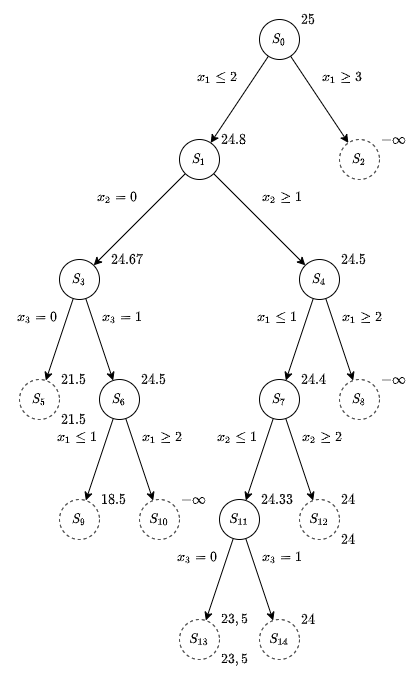
\includegraphics[width=0.8\textwidth]{figures/integer_programmin_homework_4.png}
\end{figure}

The sub-problems were explored in a breadth-first approach, so the iterations can be followed by the indices. Note that the pruned nodes are marked with dashed contour and the upper bounds found through the linear relaxations are in the top-right of each node, while the lower bound are in the bottom-right. Nodes 5, 12 and 13 were bound by optimality; nodes 2, 8 and 10 were pruned by infeasibility; and nodes 9 and 14 were pruned by bound.

All LP relaxations were solved using Gurobipy, Gurobi's interface for Python. The implementation can be seen in the \texttt{homework-4.pdf} file, which is the jupyter notebook with the python code.

\exercise{5}

The optimal solution of the LP relaxation is \[
x_1 = 0;\, x_2=1;\, x_3=\frac{3}{4}
\] with a cost of 14.5.

We write the lagrangean relaxation of the proposed 0-1 knapsack problem as
\begin{align*}
    Z(u) = \max_{x_1,x_2,x_3} \quad & 10x_1+4x_2+14x_3 + u\left( 4-3x_1-x_2-4x_3 \right)  \\
    \textrm{s.t.} \quad & x_1,x_2,x_3\in \left\{ 0,1 \right\}
\end{align*}
and the lagrangean dual as
\begin{align*}
    W_{LD} = \min_{u} \quad & Z(u) \\
    \textrm{s.t.} \quad & u\ge 0
.\end{align*}

As we have a finite and small number of feasible points $X=\left\{ x^{1},\ldots,x^{8} \right\} = \left\{ 0,1 \right\}^{3}$, the lagrangean dual was solved using Gurobi through the formulation
\begin{align*}
    \min_{\eta,u} \quad & \eta \\
    \textrm{s.t.} \quad & \eta \ge 10x_1^{t}+4x_2^{t}+14x_3^{t} + u\left( 4-3x_1^{t}-x_2^{t}-4x_3^{t} \right),\, t=1,\ldots,8  \\
      & u\in \R_+,\eta\in \R
.\end{align*}
The optimal value for the lagrangean multiplier was 3.5 with a cost of 14.5.

It is known (Theorem 10.1 of Wolsey's Integer Programming, 2021) that the lagrangean dual gives us a solution in the convex hull of the constraints not dualized. This, in our problem, can be written as \[
W_{LD} = \max\left\{ 10x_1+4x_2+14x_3 : 3x_1+x_2+4x_3\le 4,\, x\in \text{conv}\left( X \right)  \right\} 
.\] Now, note that \[
\text{conv}\left( X \right) = \left[ 0,1 \right] ^{3}
,\] which is precisely the linear relaxation of the original problem, thus why both approaches find the same optimal value.

The implementation of both approaches can be seen in \texttt{homework-5.pdf}.

\exercise{6}

\subexercise{(a)}

Let $x_i \in \left\{ 1,\ldots,n \right\} $ be the order in which task $i$ is performed. For it to be a feasible solution, no more than one task must be processed at each time, that is, \[
x_i \neq x_j ,\, i\neq j,\, i,j \in V \tag{$*$}
.\] Also, the precedence defined by $G=\left( V,E \right) $ must be respected, thus \[
x_i < x_j\,\forall \left( i,j \right) \in E \tag{$**$}
.\]

Still, one must compute the start time \[
s_i = \sum_{j \in V : x_j < x_i } p_j
,\] which is a nonlinear constraint. For us to handle this constraint, we add a support variable $y_{ij}$ which represents that task $i$ precedes task $j$. This way, with a big enough $M$ constant value, one can write
\begin{align*}
    x_i - x_j &\ge 1 - My_{ij} \\
    x_i - x_j &\le -1 + M \left( 1 -  y_{ij}\right)
.\end{align*}
Notice how these constraints also imply ($*$). Also, ($**$) can now be written \[
y_{ij} = 1\,\forall \left( i,j \right) \in E 
.\] 

Finally, we can write the problem
\begin{align*}
    \min_{x_1,\ldots,x_n} \quad & \sum_{i=1}^{n} w_i s_i \\
    \textrm{s.t.} \quad & x_i - x_j \ge 1 - My_{ij},\, i,j \in V ,\, i\neq j \\
      & x_i - x_j \le  1 - M \left( 1 - y_{ij}\right) ,\, i,j \in V ,\, i\neq j \\
      & y_{ij} = 1,\, \forall \left( i,j \right) \in E \\
      & s_i = \sum_{j \in V} p_j y_{ji} \\
      & y_{ij} \in \left\{ 0,1 \right\},\, i,j \in V \\
      & x_i \in \left\{ 1,\ldots,n \right\}
.\end{align*}

The AMPL formulation can be seen in files \texttt{ampl-6.\{mod,dat,run\}}. The problem was solved using CPLEX, in the NEOS server. The output was:

\begin{alltt}
Presolve eliminates 36 constraints and 6 variables. \\
Adjusted problem: \\
162 variables: \\
\-\hspace{2cm}138 binary variables \\
\-\hspace{2cm}12 integer variables \\
\-\hspace{2cm}12 linear variables \\
270 constraints, all linear; 918 nonzeros \\
\-\hspace{2cm}12 equality constraints \\
\-\hspace{2cm}258 inequality constraints \\
1 linear objective; 12 nonzeros. \\

CPLEX 20.1.0.0: threads=4 \\
CPLEX 20.1.0.0: optimal integer solution; objective 1888 \\
288 MIP simplex iterations \\
0 branch-and-bound nodes \\
:      \_varname  \_var    := \\
1     'x[1]'        7 \\
2     'x[2]'       10 \\
3     'x[3]'        8 \\
4     'x[4]'       12 \\
5     'x[5]'        1 \\
6     'x[6]'        5 \\
7     'x[7]'       11 \\
8     'x[8]'        4 \\
9     'x[9]'        2 \\
10    'x[10]'       6 \\
11    'x[11]'       3 \\
12    'x[12]'       9 \\
\end{alltt}


\exercise{7}

A possible formulation for the problem is to transform it into a maximum $s$-$t$ flow problem. If we assign to each edge of the graph a unitary capacity, then we will make sure that through each edge there is at most one path that goes from $s$ to $t$. Thus, the maximum flow is the number of disjoint paths that exist. This becomes clear when we consider the Ford-Fulkerson algorithm/method for computing the maximum flow of a graph, which relies on augmenting paths.

With this modification, and by adding $\left( t,s \right) $ to $E$, one can formulate the problem as
\begin{align*}
    \max_{x_{ij}} \quad & x_{ts} \\
    \textrm{s.t.} \quad & \sum_{k \in V^{+}\left( i \right) }x_{ik} - \sum_{k\in V^{-}\left( i \right) } x_{ki} = 0,\, \forall i\in V \\
      & x_{ij}\in \left\{ 0,1 \right\} ,\,\forall \left( i,j \right) \in E\setminus \left\{ \left( t,s \right)  \right\}
.\end{align*}

The AMPL formulation can be seen in files \texttt{ampl-7.\{mod,dat,run\}}. The problem was solved using CPLEX, in the NEOS server. The output was:
\begin{alltt}
Presolve eliminates 23 constraints. \\
Adjusted problem: \\
12 variables: \\
\-\hspace{2cm}11 binary variables \\
\-\hspace{2cm}1 integer variable \\
8 constraints, all linear; 24 nonzeros \\
\-\hspace{2cm}8 equality constraints \\
1 linear objective; 1 nonzero.

CPLEX 20.1.0.0: threads=4 \\
CPLEX 20.1.0.0: optimal integer solution; objective 2 \\
0 MIP simplex iterations \\
0 branch-and-bound nodes \\
:    \_varname \_var    := \\
1    'x[1,2]'   1 \\
2    'x[1,4]'   1 \\
3    'x[2,3]'   1 \\
4    'x[2,6]'   0 \\
5    'x[3,4]'   0 \\
6    'x[3,5]'   1 \\
7    'x[4,7]'   1 \\
8    'x[5,6]'   1 \\
9    'x[5,7]'   0 \\
10   'x[6,8]'   1 \\
11   'x[7,8]'   1 \\
12   'x[8,1]'   2
\end{alltt}


\end{document}
